% questions.tex —— 2011 年·重庆卷·文科 · 题目内容片段（无答案）
% 由 tools/generate_projects.py 依来源总账自 2011/2011_数学真题_重庆文_试题.md 生成，勿手改（改源 MD 后重跑）

\gkpart{一、选择题}

\begin{question}
\gkti{1}在等差数列 $\{a_n\}$ 中，$a_2=2$，$a_3=4$，则 $a_{10}=$\mbox{（　　）}

（A）$12$

（B）$14$

（C）$16$

（D）$18$

\end{question}
\begin{question}
\gkti{2}设 $U=\mathbf R$，$M=\{x\mid x^2-2x>0\}$，则 $\complement_U M=$\mbox{（　　）}

（A）$[0,2]$

（B）$(0,2)$

（C）$(-\infty,0)\cup(2,+\infty)$

（D）$(-\infty,0]\cup[2,+\infty)$

\end{question}
\begin{question}
\gkti{3}曲线 $y=-x^3+3x^2$ 在点 $(1,2)$ 处的切线方程为\mbox{（　　）}

（A）$y=3x-1$

（B）$y=-3x+5$

（C）$y=3x+5$

（D）$y=2x$

\end{question}
\begin{question}
\gkti{4}从一堆苹果中任取 $10$ 只，称得它们的质量如下（单位：克）：

\nopagebreak[4]
\[125\quad120\quad122\quad105\quad130\quad114\quad116\quad95\quad120\quad134\]

则样本数据落在 $[114.5,124.5]$ 内的频率为\mbox{（　　）}

（A）$0.2$

（B）$0.3$

（C）$0.4$

（D）$0.5$

\end{question}
\begin{question}
\gkti{5}已知向量 $\boldsymbol a=(1,k)$，$\boldsymbol b=(2,2)$，且 $\boldsymbol a+\boldsymbol b$ 与 $\boldsymbol a$ 共线，那么 $\boldsymbol a\cdot\boldsymbol b$ 的值为\mbox{（　　）}

（A）$1$

（B）$2$

（C）$3$

（D）$4$

\end{question}
\begin{question}
\gkti{6}设 $a=\log_{\frac13}\dfrac12$，$b=\log_{\frac13}\dfrac23$，$c=\log_3\dfrac43$，则 $a$，$b$，$c$ 的大小关系是\mbox{（　　）}

（A）$a<b<c$

（B）$c<b<a$

（C）$b<a<c$

（D）$b<c<a$

\end{question}
\begin{question}
\gkti{7}若函数 $f(x)=x+\dfrac1{x-2}$（$x>2$）在 $x=a$ 处取最小值，则 $a=$\mbox{（　　）}

（A）$1+\sqrt2$

（B）$1+\sqrt3$

（C）$3$

（D）$4$

\end{question}
\begin{question}
\gkti{8}若 $\triangle ABC$ 的内角 $A$、$B$、$C$ 满足 $6\sin A=4\sin B=3\sin C$，则 $\cos B=$\mbox{（　　）}

（A）$\dfrac{\sqrt{15}}4$

（B）$\dfrac34$

（C）$\dfrac{3\sqrt{15}}{16}$

（D）$\dfrac{11}{16}$

\end{question}
\begin{question}
\gkti{9}设双曲线的左准线与两条渐近线交于 $A$、$B$ 两点，左焦点在以 $AB$ 为直径的圆内，则该双曲线的离心率取值范围为\mbox{（　　）}

（A）$\left(0,\sqrt2\right)$

（B）$\left(1,\sqrt2\right)$

（C）$\left(\dfrac{\sqrt2}2,1\right)$

（D）$\left(\sqrt2,+\infty\right)$

\end{question}
\begin{question}
\gkti{10}高为 $\sqrt2$ 的四棱锥 $S-ABCD$ 的底面是边长为 $1$ 的正方形，点 $S$、$A$、$B$、$C$、$D$ 均在半径为 $1$ 的同一球面上，则底面 $ABCD$ 的中心与顶点 $S$ 之间的距离为\mbox{（　　）}

（A）$\dfrac{\sqrt{10}}2$

（B）$\dfrac{\sqrt2+\sqrt3}2$

（C）$\dfrac32$

（D）$\sqrt2$

\end{question}
\gkpart{二、填空题}

\begin{question}
\gkti{11}$(1+2x)^6$ 的展开式中 $x^4$ 的系数是 $\underline{\qquad}$。

\end{question}
\begin{question}
\gkti{12}若 $\cos\alpha=-\dfrac35$，且 $\alpha\in\left(\pi,\dfrac{3\pi}2\right)$，则 $\tan\alpha=\underline{\qquad}$。

\end{question}
\begin{question}
\gkti{13}过原点的直线与圆 $x^2+y^2-2x-4y+4=0$ 相交所得弦的长为 $2$，则该直线的方程为 $\underline{\qquad}$。

\end{question}
\begin{question}
\gkti{14}从甲、乙等 $10$ 位同学中任选 $3$ 位去参加某项活动，则所选 $3$ 位中有甲但没有乙的概率为 $\underline{\qquad}$。

\end{question}
\begin{question}
\gkti{15}若实数 $a$，$b$，$c$ 满足 $2^a+2^b=2^{a+b}$，$2^a+2^b+2^c=2^{a+b+c}$，则 $c$ 的最大值是 $\underline{\qquad}$。

\end{question}
\gkpart{三、解答题}

\begin{question}
\gkti{16}设 $\{a_n\}$ 是公比为正数的等比数列，$a_1=2$，$a_3=a_2+4$。

（1） 求 $\{a_n\}$ 的通项公式；

（2） 设 $\{b_n\}$ 是首项为 $1$，公差为 $2$ 的等差数列，求数列 $\{a_n+b_n\}$ 的前 $n$ 项和 $S_n$。

\end{question}
\begin{question}
\gkti{17}某市公租房的房源位于 $A$、$B$、$C$ 三个片区。设每位申请人只申请其中一个片区的房源，且申请其中任一个片区的房源是等可能的，求该市的任 $4$ 位申请人中：

（1） 没有人申请 $A$ 片区房源的概率；

（2） 每个片区的房源都有人申请的概率。

\end{question}
\begin{question}
\gkti{18}设函数 $f(x)=\sin x\cos x-\sqrt3\cos(\pi+x)\cos x$（$x\in\mathbf R$）。

（1） 求 $f(x)$ 的最小正周期；

（2） 若函数 $y=f(x)$ 的图象按 $\boldsymbol b=\left(\dfrac\pi4,\dfrac{\sqrt3}2\right)$ 平移后得到函数 $y=g(x)$ 的图象，求 $y=g(x)$ 在 $\left[0,\dfrac\pi4\right]$ 上的最大值。

\end{question}
\begin{question}
\gkti{19}设 $f(x)=2x^3+ax^2+bx+1$ 的导数为 $f'(x)$，若函数 $y=f'(x)$ 的图象关于直线 $x=-\dfrac12$ 对称，且 $f'(1)=0$。

（1） 求实数 $a$，$b$ 的值；

（2） 求函数 $f(x)$ 的极值。

\Needspace{0.4\textheight}
\end{question}
\begin{question}
\gkti{20}如图，在四面体 $ABCD$ 中，平面 $ABC\perp$ 平面 $ACD$，$AB\perp BC$，$AC=AD=2$，$BC=CD=1$。

（1） 求四面体 $ABCD$ 的体积；

（2） 求二面角 $C-AB-D$ 的平面角的正切值。
\nopagebreak[4]
\begin{center}% 2011 年重庆卷文科第 20 题：四面体 ABCD，平面 ABC⊥平面 ACD。
% 来源 PDF：普通高考/2011/2011重庆文.pdf，SHA-256 0ddbe738e4414213612fb6f62ec0c5cd252d039abf560bae1f31610558f93a70。
% 原页：第 2 页第 2 栏上部，书页码 654。示意。
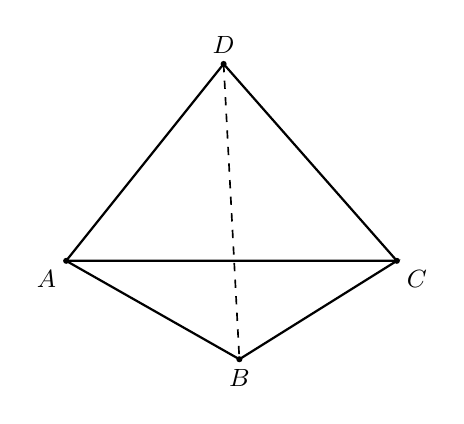
\begin{tikzpicture}[>=stealth, semithick, font=\small, scale=1.0]
  \coordinate (A) at (0,0);
  \coordinate (C) at (4.2,0);
  \coordinate (B) at (2.2,-1.25);
  \coordinate (D) at (2.0,2.5);
  \draw[thick] (A)--(B)--(C)--(A);
  \draw[thick] (D)--(A) (D)--(C);
  \draw[dashed] (D)--(B);
  \fill (A) circle (1.1pt) node[below left] {$A$};
  \fill (B) circle (1.1pt) node[below] {$B$};
  \fill (C) circle (1.1pt) node[below right] {$C$};
  \fill (D) circle (1.1pt) node[above] {$D$};
\end{tikzpicture}
\end{center}
\nopagebreak[4]
\Needspace{0.4\textheight}
\end{question}
\begin{question}
\gkti{21}如图，椭圆的中心为原点 $O$，离心率 $e=\dfrac{\sqrt2}2$，一条准线的方程是 $x=2\sqrt2$。

（1） 求该椭圆的标准方程；

（2） 设动点 $P$ 满足 $\overrightarrow{OP}=\overrightarrow{OM}+2\overrightarrow{ON}$，其中 $M$，$N$ 是椭圆上的点，直线 $OM$ 与 $ON$ 的斜率之积为 $-\dfrac12$，问：是否存在定点 $F$，使得 $|PF|$ 与点 $P$ 到直线 $l:x=2\sqrt{10}$ 的距离之比为定值？若存在，求 $F$ 的坐标；若不存在，说明理由。
\nopagebreak[4]
\begin{center}% 2011 年重庆卷文科第 21 题：椭圆、准线 x=2√2 与点 P、M、N。
% 来源 PDF：普通高考/2011/2011重庆文.pdf，SHA-256 0ddbe738e4414213612fb6f62ec0c5cd252d039abf560bae1f31610558f93a70。
% 原页：第 2 页第 3 栏中部，书页码 654。示意。
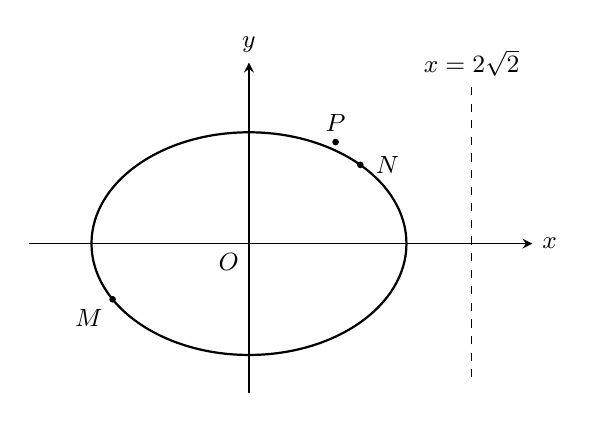
\begin{tikzpicture}[>=stealth, semithick, font=\small, scale=1.0]
  \draw[->] (-2.8,0)--(3.6,0) node[right] {$x$};
  \draw[->] (0,-1.9)--(0,2.3) node[above] {$y$};
  \draw[thick] (0,0) ellipse (2 and 1.414);
  \draw[dashed] (2.828,-1.7)--(2.828,2.0) node[above] {$x=2\sqrt2$};
  \fill (-1.732,-0.707) circle (1.2pt) node[below left] {$M$};
  \fill (1.414,1.0) circle (1.2pt) node[right=2pt] {$N$};
  \fill (1.10,1.29) circle (1.2pt) node[above] {$P$};
  \node[below left] at (0,0) {$O$};
\end{tikzpicture}
\end{center}
\nopagebreak[4]

\end{question}